\documentclass{article}
\usepackage{enumitem}
\usepackage{graphicx}
\graphicspath{{images/}}

\begin{document}
\begin{enumerate}[label=\textbf{\Alph*.}]
	\item .\\
	\begin{figure}[h]
		\centering
		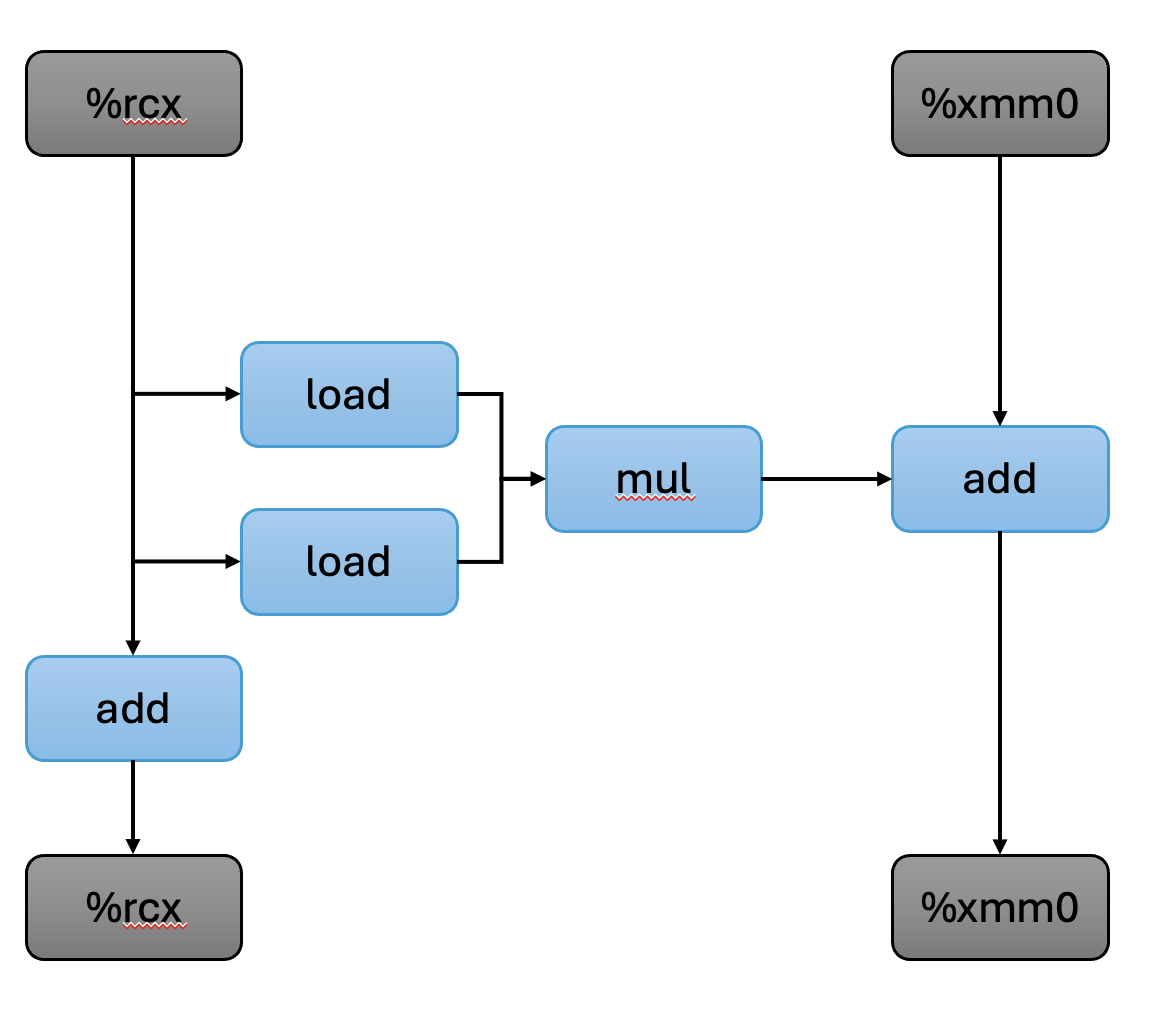
\includegraphics[width=0.75\textwidth]{fig1}
		\caption{Data flow figure}
		\label{fig:fig1}
	\end{figure} \\
	As you can see in figure \ref{fig:fig1}, the data in the register \%|xmm0 in
	previous iteration will be reused in the next iteration.
	\item For data type double, what lower bound on the CPE is determined by the
	critical path? \\
	The only operation on the critical path is floating point addition with CPE of
	3.0.
	\item . \\
	1.0
	\item . \\
	The result of multiplication can be calculated previously before it used in
	the accumulator.
\end{enumerate}
\end{document}
